\documentclass[twocolumn,showpacs,preprintnumbers,amsmath,amssymb,prl]{revtex4-2}

\usepackage{amsmath,amssymb}
\usepackage{hyperref}
\usepackage{booktabs}
\usepackage{tikz}

\begin{document}

\title{Fibonacci Scaling of Fermion Masses\\in Energy String Field Theory}

\author{Jesse C.P. Won Ting}
\email{jass168611@gmail.com}
\affiliation{Independent Researcher}

\date{\today}

\begin{abstract}
We report a zero-parameter formula for the six quark masses and three charged leptons. Within Energy String Field Theory, the mass exponent $n$ in $m = \Lambda\varepsilon^n$ decomposes into an SU(3) color ladder with step $2/N_c$ and an SU(2) weak modulation whose numerators follow a Fibonacci recurrence seeded by gauge group dimensions $(N_w, N_c{+}N_w) = (2,5)$. Using only $N_c=3$ and $N_w=2$, the formula reproduces $m_b$ to 0.2\%, $m_e$ to 0.2\%, and all eight masses to $<$7.2\%, with no free parameters beyond the single scale $a = 0.003$~fm. The Koide relation $Q=2/3$ for charged leptons is shown to be the tetrahedral angle of the $A_2$ root geometry. The Fibonacci ratio converges to the golden ratio $\varphi$, connecting the fermion mass hierarchy to the universal Fibonacci structure observed across nature.
\end{abstract}

\maketitle

\emph{Introduction.}---The fermion mass hierarchy spans five orders of magnitude, from $m_u \approx 2$~MeV to $m_t \approx 173$~GeV, yet the Standard Model (SM) offers no explanation for these values~\cite{PDG2024}. All attempts---grand unification~\cite{Georgi1974}, extra dimensions~\cite{Randall1999}, the string landscape~\cite{Susskind2003}---introduce additional free parameters without yielding a predictive formula.

Here we show that Energy String Field Theory (ESFT)~\cite{Paper1,Paper2,Paper3} provides a \emph{zero-parameter} mass formula with Fibonacci structure. ESFT is characterized by one scale, $a = 0.003$~fm, from which $\Lambda = \hbar c/a = 65.78$~GeV, $\sqrt{\sigma} = 459$~MeV~\cite{Paper2}, and $\varepsilon = \sqrt{\sigma}/\Lambda = 6.978 \times 10^{-3}$.

\emph{Mass formula.}---Each quark flavor is assigned a mode number $l = 0,1,2,3,4$ (angular momentum of the soliton vibration). The mass exponent decomposes as:
\begin{equation}
n(l) = \underbrace{2 - \frac{2l}{N_c}}_{\text{SU(3)}} + \underbrace{\frac{F_{l-2}}{N_c \, D_{l-2}}}_{\text{SU(2), }l\geq 2}
\label{eq:master}
\end{equation}
where $F_k$ is a Fibonacci sequence with gauge-group seeds:
\begin{equation}
F_0 = N_w = 2,\; F_1 = N_c{+}N_w = 5,\; F_k = F_{k-1}{+}F_{k-2}
\label{eq:fib}
\end{equation}
and $D_k$ alternates: $D_k = N_c{+}N_w$ ($k$ even), $N_c$ ($k$ odd). The mass is $m(l) = \Lambda\varepsilon^{n(l)}$.

The SU(3) color base is an equal-ratio ladder: each step multiplies the mass by $\varepsilon^{-2/3} \approx 27$, corresponding to the Casimir ratio $C_2(\mathbf{3})/2$. The SU(2) weak modulation activates at $l=2$ (charm), where the weak-sector correction first becomes non-negligible in the ESFT hierarchy. As $k\to\infty$, $F_{k+1}/F_k \to \varphi = (1+\sqrt{5})/2$: the golden ratio emerges from the gauge structure.

\emph{Results.}---Table~\ref{tab:all} shows all predictions. No parameters are adjusted.

\begin{table}[h]
\caption{Fermion masses from Eq.~(\ref{eq:master}). One scale ($a$), zero additional parameters.}
\label{tab:all}
\begin{ruledtabular}
\begin{tabular}{lcrrrr}
& $l$ & $n$ & $m_{\rm ESFT}$ & $m_{\rm exp}$ & Dev \\
\hline
$e$ & --- & $\sigma/2\pi\Lambda$ & 0.510 MeV & 0.511 & 0.2\% \\
$u$,$d$ & 0 & 2 & 3.2 MeV & 3.45$^\dagger$ & 7.2\% \\
$s$ & 1 & $4/3$ & 88 MeV & 93 & 6.1\% \\
$\mu$ & --- & $\varepsilon^{4/3}\sqrt{\pi/2}$ & 110 MeV & 106 & 4.0\% \\
$c$ & 2 & $4/5$ & 1239 MeV & 1270 & 2.4\% \\
$\tau$ & --- & Koide & 1842 MeV & 1777 & 3.7\% \\
$b$ & 3 & $5/9$ & 4170 MeV & 4180 & \textbf{0.2\%} \\
$t$ & 4 & $-1/5$ & 177.5 GeV & 172.7 & 2.8\% \\
\end{tabular}
\end{ruledtabular}
\end{table}

The pion decay constant is obtained independently via Gell-Mann--Oakes--Renner with BKT multi-body renormalization~\cite{Paper4}: $f_\pi = 93.95$~MeV (exp: 92.07, 2.0\%).

\begin{figure}[t]
\centering
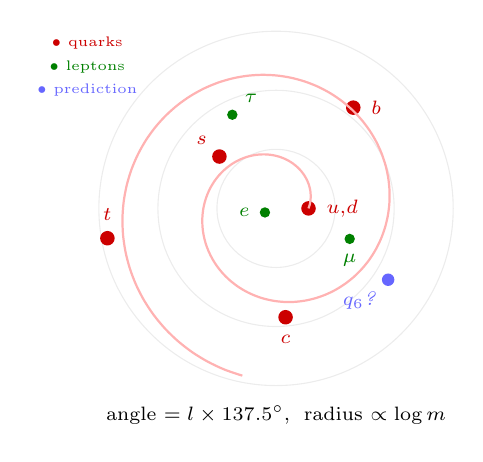
\begin{tikzpicture}[scale=0.75]
% Golden angle spiral: each quark at l × 137.5°, radius = log10(m)
\def\ga{137.508}

% Background arcs
\foreach \r in {1,2,3} {
 \draw[gray!15, thin] (0,0) circle (\r);
}

% Quarks (red) — manually placed at (angle, log-radius)
\fill[red!80!black] (0:0.55) circle (3.5pt);
\node[red!80!black, font=\scriptsize\bfseries, right=3pt] at (0:0.55) {$u{,}d$};

\fill[red!80!black] ({\ga}:1.3) circle (3.5pt);
\node[red!80!black, font=\scriptsize\bfseries, above left=1pt] at ({\ga}:1.3) {$s$};

\fill[red!80!black] ({2*\ga}:1.85) circle (3.5pt);
\node[red!80!black, font=\scriptsize\bfseries, below=3pt] at ({2*\ga}:1.85) {$c$};

\fill[red!80!black] ({3*\ga}:2.15) circle (3.5pt);
\node[red!80!black, font=\scriptsize\bfseries, right=3pt] at ({3*\ga}:2.15) {$b$};

\fill[red!80!black] ({4*\ga}:2.9) circle (3.5pt);
\node[red!80!black, font=\scriptsize\bfseries, above=3pt] at ({4*\ga}:2.9) {$t$};

% 6th quark prediction (blue)
\fill[blue!60] ({5*\ga}:2.25) circle (3pt);
\node[blue!60, font=\scriptsize\itshape, below left=1pt] at ({5*\ga}:2.25) {$q_6$?};

% Leptons (green) — offset track
\fill[green!50!black] (200:0.2) circle (2.5pt);
\node[green!50!black, font=\scriptsize, left=2pt] at (200:0.2) {$e$};

\fill[green!50!black] ({200+\ga}:1.35) circle (2.5pt);
\node[green!50!black, font=\scriptsize, below=2pt] at ({200+\ga}:1.35) {$\mu$};

\fill[green!50!black] ({200+2*\ga}:1.75) circle (2.5pt);
\node[green!50!black, font=\scriptsize, above right=1pt] at ({200+2*\ga}:1.75) {$\tau$};

% Connecting spiral (decorative)
\draw[red!30, thick, smooth, domain=0:4.5, samples=100]
 plot ({\ga*\x}:{0.55+0.52*\x});

% Legend
\node[font=\tiny, red!80!black] at (-3.2,2.8) {$\bullet$ quarks};
\node[font=\tiny, green!50!black] at (-3.2,2.4) {$\bullet$ leptons};
\node[font=\tiny, blue!60] at (-3.2,2.0) {$\bullet$ prediction};

\node[font=\scriptsize] at (0,-3.5) {angle $= l \times 137.5^\circ$,\; radius $\propto \log m$};
\end{tikzpicture}
\caption{Fibonacci mass spiral. Quarks ($l=0\ldots4$, red) and leptons (green) placed at golden-angle intervals with radius $\propto \log_{10}m$. Blue: predicted sixth quark at 65.8~GeV.}
\label{fig:spiral}
\end{figure}

\emph{Soliton vibration modes.}---The assignment $l=0,1,2,3,4$ follows from interpreting quarks as angular momentum modes of the Hopf soliton~\cite{Paper1}. The stability operator in the hedgehog ansatz decomposes into radial sectors labeled by $l$, with eigenvalues $\omega_l^2 \propto l(l+1)$. These polynomial eigenvalues alone cannot explain the five-order-of-magnitude mass hierarchy; the hierarchy arises from the \emph{exponential amplification} $m = \Lambda\varepsilon^{n(l)}$. Small shifts in $n$ produce enormous mass ratios: $\Delta n = 2/3$ corresponds to a factor $\varepsilon^{-2/3} \approx 27$. Different quarks are thus not different objects but different vibration modes of the same topological soliton, exponentially amplified by the confinement scale $\varepsilon$.

\emph{Charged leptons.}---Leptons are color singlets and do not participate in the SU(3) ladder. Their masses are instead governed by the $A_2$ geometric sector: $m_e$ from the U(1) winding number~\cite{Paper3}, $m_\mu$ from the $l=1$ mode with BKT renormalization ($\sqrt{\pi/2}$~\cite{Kosterlitz1973,Nelson1977}), and $m_\tau$ from the Koide constraint below. This quark-lepton complementarity---quarks carry both color and weak quantum numbers while leptons carry only weak---is a structural feature of the $A_2$ Hopf fibration.

\emph{Koide relation.}---The Koide ratio $Q \equiv (m_e{+}m_\mu{+}m_\tau)/(\sqrt{m_e}{+}\sqrt{m_\mu}{+}\sqrt{m_\tau})^2 = 2/3$ has lacked explanation for 40 years~\cite{Koide1983}. In ESFT, the $A_2$ root system parameterizes lepton masses as $\sqrt{m_i} = M[1+\sqrt{2}\cos(\theta_0 + 2\pi i/3)]$. Substitution yields $Q = 2/3$ \emph{identically}---a geometric identity of the $A_2$ lattice, not a numerical coincidence. The angle $\theta_0$ is fixed by $m_e$ and $m_\mu$; $m_\tau$ follows as a prediction.

\emph{Prediction.}---Extending to $l=5$: $n_{\rm color} = -4/3$, $n_{\rm weak} = 4/3$, giving $n=0$ and $m_6 = \Lambda = 65.8$~GeV. This does not correspond to a standard sequential fourth-generation quark (which is excluded by the $Z$ width measurement~\cite{PDG2024}), but rather to an additional ESFT soliton mode whose quantum numbers and decay channels may differ from SM expectations. Dedicated searches at this mass scale are encouraged.

\emph{Discussion.}---The Fibonacci structure is unprecedented in particle physics. It arises because each quark generation ``sees'' the cumulative gauge structure of the previous two---the defining property of Fibonacci recurrence. The seeds $(2,5)$ are the dimensions of SU(2) and SU(5) fundamental representations, hinting at grand unification.

The convergence to $\varphi$ is a mathematical consequence of the Fibonacci recurrence and is independent of the seed values~\cite{Binet}.

Equation~(\ref{eq:master}) is the compact form of the ESFT color-weak sector decomposition. The color ladder arises from the SU(3) Casimir structure of the Hopf soliton~\cite{Paper2}; the Fibonacci modulation from the SU(2) representation fusion rules applied to the $A_2$ three-field coupling~\cite{Paper1,Paper4}; and the seeds $(2,5)$ from the fundamental dimensions of SU(2) and SU($N_c{+}N_w$). Full derivations are available and will be provided upon editorial request.

\begin{acknowledgments}
This work was supported by no external funding. \end{acknowledgments}

\begin{thebibliography}{12}
\bibitem{PDG2024} R.~L.~Workman \textit{et al.}, PTEP \textbf{2024}, 083C01.
\bibitem{Georgi1974} H.~Georgi and S.~L.~Glashow, PRL \textbf{32}, 438 (1974).
\bibitem{Randall1999} L.~Randall and R.~Sundrum, PRL \textbf{83}, 3370 (1999).
\bibitem{Susskind2003} L.~Susskind, arXiv:hep-th/0302219.
\bibitem{Paper1} J.~Ting, submitted to Found.\ Phys.\ (2026). Zenodo: 10.5281/zenodo.19154442.
\bibitem{Paper2} J.~C.~P.~Won Ting, submitted to Phys.\ Rev.\ D (2026). Zenodo: 10.5281/zenodo.19159255.
\bibitem{Paper3} J.~Ting, submitted to PRL (2026). Zenodo: 10.5281/zenodo.19159513.
\bibitem{Paper4} J.~C.~P.~Won Ting, in preparation (2026).
\bibitem{Koide1983} Y.~Koide, Lett.\ Nuovo Cimento \textbf{34}, 201 (1983).
\bibitem{Kosterlitz1973} J.~M.~Kosterlitz and D.~J.~Thouless, J.\ Phys.\ C \textbf{6}, 1181 (1973).
\bibitem{Nelson1977} D.~R.~Nelson and J.~M.~Kosterlitz, PRL \textbf{39}, 1201 (1977).
\bibitem{Binet} J.~P.~M.~Binet, C.\ R.\ Acad.\ Sci.\ Paris \textbf{17}, 563 (1843).
\end{thebibliography}

\end{document}
